\section{Semaine 14 : 08/05/2023 - 12/05/2023}
\graphicspath{{semaines/semaine_14/images/}}

%On va également tester de faire une IPP sur le second membre $\tilde{f}$ pour n'utiliser que les dérivées premières de $\tilde{\phi}$. On comparera les résultats avec et sans IPP.

\begin{abstract}
	On souhaite faire fonctionner le rehaussement avec PhiFEM en utilisant la méthode duale. On commencera par faire les courbes de convergence puis on comparera pour différent cas tests, les erreurs en norme $L^2$ des méthodes suivantes : $\Phi$-FEM par méthode directe, $\Phi$-FEM par méthode duale, Correction par multiplication sans rehaussement, Correction par multiplication avec rehaussement par méthode duale, Correction par addition.
	
	Après discussion avec Emmanuel, il semblerait que les résultats obtenus pour $\tilde{\phi}$ de degré 2 ne soient pas aberrant. On va alors continuer les tests sur le FNO en lui appliquant les mêmes méthodes de correction que celles testées sur la solution analytique.
	
	Après relecture du document sur le rehaussement par Michel, il m'a demandé de faire la théorie sur l'erreur d'interpolation mis dans le document pour le rehaussement (inégalité 7 qui m'avait été dite par Emmanuel). Jeudi, on a alors discuté de ça avec Michel et vendredi j'ai alors relu ce que Michel avait fait pour essayer de bien comprendre.
\end{abstract}

\subsection{Présentation : méthode duale pour $\phi$-FEM}

On considère le problème de Poisson avec condition de Dirichlet homogène ou non homogène :
\begin{equation*}
	\left\{\begin{aligned}
		&-\Delta u=f \quad &&\Omega \\
		&u=g \quad &&\Gamma
	\end{aligned}\right.
\end{equation*}

La formulation variationnelle PhiFEM pour ce problème en utilisant la méthode duale est :

$$\int_{\Omega_h}\nabla u\nabla v-\int_{\partial\Omega_h}\frac{\partial u}{\partial n} v + \frac{\gamma}{h^2} \sum_{T\in\mathcal{T}_h^\Gamma}\int_T \left(u-\frac{1}{h}\phi p\right)\left(v-\frac{1}{h}\phi q\right) + G_h(u,v) = \int_{\Omega_h}fv + \frac{\gamma}{h^2} \sum_{T\in\mathcal{T}_h^\Gamma}\int_T g\left(v-\frac{1}{h}\phi q\right) + G_h^{rhs}(v)$$
avec
$$G_h(u,v)=\sigma h\sum_{E\in\mathcal{F}_h^\Gamma}\int_E\left[\frac{\partial u}{\partial n}\right]\left[\frac{\partial v}{\partial n}\right]+\sigma h^2\sum_{T\in\mathcal{T}_h^\Gamma}\int_T \Delta u\Delta v$$
et
$$G_h^{rhs}(v)=-\sigma h^2\sum_{T\in\mathcal{T}_h^\Gamma}\int_T f\Delta v$$

Pour la correction, on considère le problème suivant :

\begin{equation*}
	\left\{\begin{aligned}
		&-\Delta (\hat{\phi}C)=f \quad &&\Omega \\
		&\hat{u}=g+m \quad &&\Gamma
	\end{aligned}\right. \label{pbc1r}
\end{equation*}
avec $\hat{u}=\hat{\phi}C+m$ où $\hat{\phi}=\tilde{\phi}+m$ ($m$ une constante).

La formulation variationnelle PhiFEM pour ce problème en utilisant la méthode duale est :
\begin{align*}
	\int_{\Omega_h}\nabla(\hat{\phi}C)\nabla(\hat{\phi}v)-\int_{\partial\Omega_h}\frac{\partial}{\partial n}(\hat{\phi}C)\hat{\phi}v + \frac{\gamma}{h^2} \sum_{T\in\mathcal{T}_h^\Gamma}\int_T \left(\hat{\phi} C-\frac{1}{h}\phi p\right)\left(\hat{\phi}v-\frac{1}{h}\phi q\right) + G_h(C,v)& \\
	= \int_{\Omega_h}f\hat{\phi}v + \frac{\gamma}{h^2} \sum_{T\in\mathcal{T}_h^\Gamma}\int_T (g+m)\left(\hat{\phi}v-\frac{1}{h}\phi q\right) + G_h^{rhs}(v)&
\end{align*}
avec
$$G_h(C,v)=\sigma h\sum_{E\in\mathcal{F}_h^\Gamma}\int_E\left[\frac{\partial}{\partial n}(\hat{\phi}C)\right]\left[\frac{\partial}{\partial n}(\hat{\phi}v)\right]+\sigma h^2\sum_{T\in\mathcal{T}_h^\Gamma}\int_T \Delta(\hat{\phi}C)\Delta(\hat{\phi}v)$$
et
$$G_h^{rhs}(v)=-\sigma h^2\sum_{T\in\mathcal{T}_h^\Gamma}\int_T f\Delta(\hat{\phi}v)$$

\newpage

\subsubsection*{Résultats}

On considère $\Omega$ le cercle de rayon $\sqrt{2}/4$ et de centre $(0.5,0.5)$. On prend 
$$\phi(x,y)=-1/8+(x-1/2)^2+(y-1/2)^2$$
On considère le domaine fictif $O=(0,1)^2$.


On considère toujours la solution analytique suivante :
$$u_{ex}(x,y) = S\times\sin(2\pi fx + \varphi)\times\sin(2\pi fy + \varphi)$$ 

On prend dans ce cas la perturbation $P$ définie par
$$P(x,y) = S\times\sin(2\pi fx + \varphi)\times\sin(2\pi fy + \varphi)\times\cos(4\pi((x-0.5)^2+(y-0.5)^2))$$ 
pour que $P=0$ sur $\Gamma$ (et donc $u_p=u_{ex}$ sur $\Gamma$). \\

\underline{Résultats de convergence :} \\

On cherchera à comparer pour un seul cas test les erreurs en norme $L^2$ et $H^1$ de $\phi$-FEM (sans correction) en utilisant la méthode duale, de la correction avec un rehaussement en utilisant la méthode duale et l'erreur FEM standard (sans correction). On prendra $S=S_p=0.5$, $f=4$, $f_p=2$ et $p=p_p=0$ (à noter que sur le cercle ce problème n'est pas homogène). On choisit $\epsilon=1e-2$ et $m=1000$ pour le rehaussement. On prendra $degV=1$ et $degPhi=degV+1$. Voici les résultats obtenus pour différentes tailles de maillage $h$ :

\begin{minipage}{0.38\linewidth}
	\centering
	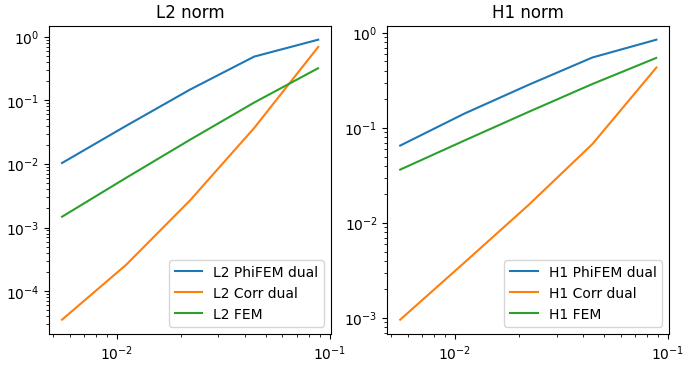
\includegraphics[width=\linewidth]{dual_courbes.png}
\end{minipage}
\begin{minipage}{0.58\linewidth}
	\centering
	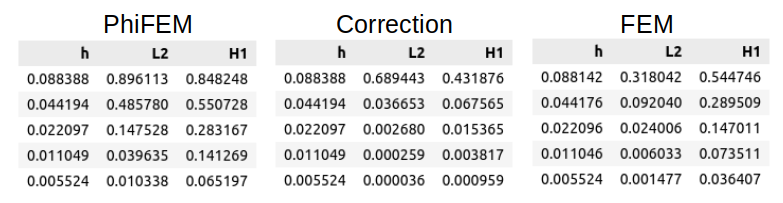
\includegraphics[width=\linewidth]{dual_results.png}
\end{minipage} \\

\underline{Comparaison des méthodes :} \\

On cherche cette fois-ci à compléter le document de la semaine dernière pour $\phi$-FEM en comparant les erreurs en norme $L^2$ pour les méthodes suivantes : $\Phi$-FEM par méthode directe, $\Phi$-FEM par méthode duale, Correction par multiplication sans rehaussement ($\tilde{u} = \tilde{\phi}C$), Correction par multiplication avec rehaussement par méthode duale ($\tilde{u} = \tilde{\phi}C+m$), Correction par addition ($\tilde{u}=\tilde{\phi}+\phi C$).  

\begin{Rem}
	On prendra ici $\tilde{\phi}$ de degré 10 et $\sigma=\gamma=20$.
\end{Rem}

\begin{minipage}{\linewidth}
	\centering
	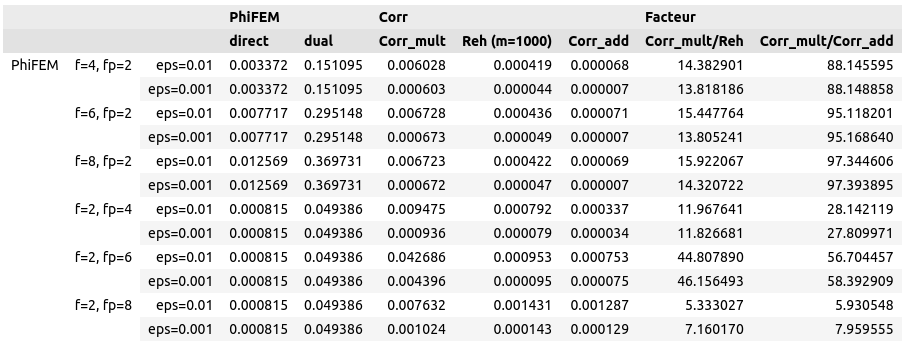
\includegraphics[width=0.6\linewidth]{comp_meth_results.png}
\end{minipage}

\begin{minipage}{\linewidth}
	\centering
	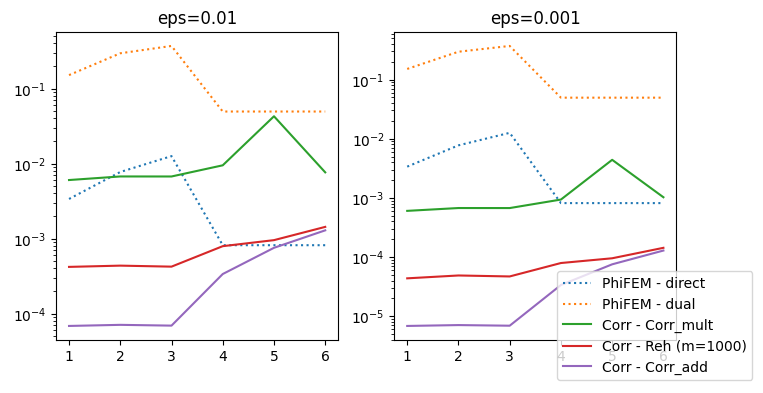
\includegraphics[width=0.5\linewidth]{comp_meth_courbes.png}
\end{minipage}

\subsection{Résultats FNO}

On considère le problème de Poisson avec condition de Dirichlet homogène :
\begin{equation*}
	\left\{\begin{aligned}
		&-\Delta u=f \quad &&\Omega \\
		&u=0 \quad &&\Gamma
	\end{aligned}\right.
\end{equation*}

On considère cette fois-ci $f$ gaussienne :
$$f(x,y) = \exp\left(-\frac{(x-\mu_0)^2 + (y-\mu_1)^2}{2\sigma^2}\right)\,, $$ 
avec $\sigma \sim \mathcal{U}([0.1,0.6])$ et $\mu_0, \mu_1 \sim \mathcal{U}([0.5-\sqrt{2}/4, 0.5+\sqrt{2}/4])$ à condition que $\phi(\mu_0, \mu_1) < -0.05$.

On considère la solution de référence $u_{ref}$ comme étant une solution sur-raffinée $\mathbb{P}^1$ obtenue par les EF standard (avec $h_{ref}\approx 0.006$ car $h_{ref}<<h_{FNO}$). \\

On cherche à appliquer sur le FNO les 3 "types " de correction : Correction par multiplication sans rehaussement ($\tilde{u} = \tilde{\phi}C$), Correction par multiplication avec rehaussement par méthode duale ($\tilde{u} = \tilde{\phi}C+m$), Correction par addition ($\tilde{u}=\tilde{\phi}+\phi C$).

\subsubsection*{Erreurs en norme $L^2$ à différentes epochs}

\begin{minipage}{\linewidth}
	\centering
	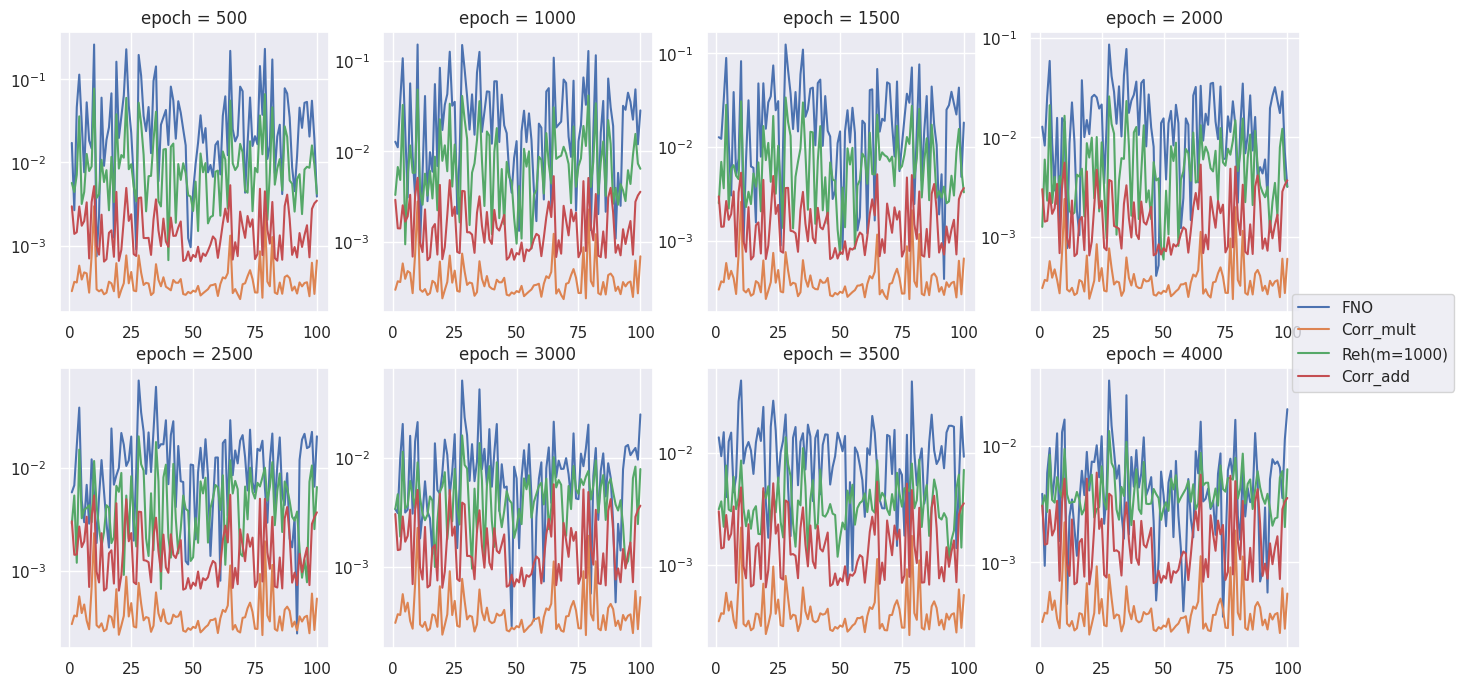
\includegraphics[width=0.7\linewidth]{FNO_errors.png}
\end{minipage}

\subsubsection*{Représentation en boxplots}

\begin{minipage}{\linewidth}
	\centering
	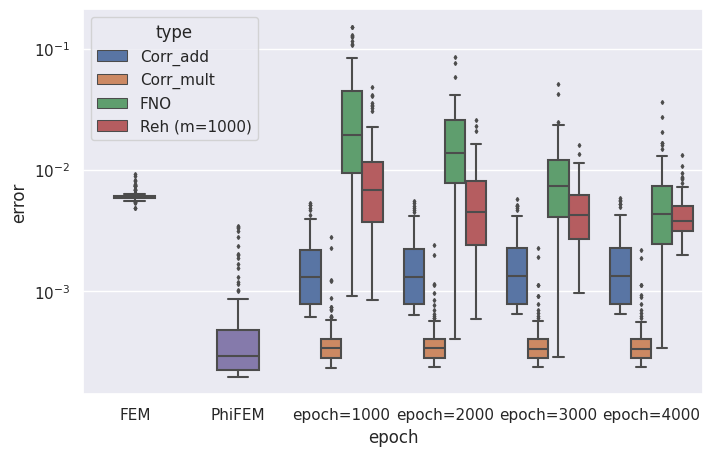
\includegraphics[width=0.5\linewidth]{FNO_boxplots.png}
\end{minipage}

\conclusion{Plusieurs autres idées de tests ont été proposé par Michel et Emmanuel. Ces tests seront expliqué dans le Résumé de la semaine prochaine. La semaine prochaine, il faudra également continuer la théorie sur le rehaussement en posant quelques questions à Michel.

Vanessa a également proposée une nouvelle idée qui consiste à combiner les deux méthodes de correction, en posant quelque chose comme $\tilde{f}=\hat{\phi}C_1+C_2$. Il semblerait d'après Michel et Killian que le problème soit mal posé.}
